\documentclass{article}
\usepackage[T1]{fontenc}
\usepackage{lmodern}
\usepackage{graphicx}
\usepackage{amsmath,amssymb}
\usepackage[a4paper,margin=2cm]{geometry}
\usepackage[absolute,overlay]{textpos}
\setlength{\TPHorizModule}{1mm}
\setlength{\TPVertModule}{1mm}
\usepackage[indonesian]{babel}
\usepackage{hyperref}
\setlength{\emergencystretch}{2em}
% unit: Halaman 24

\begin{document}

% === Halaman 24 (python/native) ===

Penggunaan OTP pada perang dingin 

antara AS dan Uni Soviet

The Moscow–Washington hotline [1963]:

•

Komunikasi antara AS dan Uni Soviet 

menggunakan hotline komunikasi langsung antara 

pemimpin AS dan Uni Soviet.

•

Hotline difasilitasi dengan peralatan OTP yang 

bernama ITT Intelex Teletype L015

•

ITT Intelex Teletype dikembangkan setelah krisis 

rudal Cuba untuk menghindari perang nuklir

•

ITT Intelex Teletype mengenkripsi pesan 

menggunakan OTP 

•

Kunci one-time pad disimpan di dalam pita 

magnetic yang diterbangkan antara  

Washington DC dan Moscow.

ITT Intelex Teletype L015 used for 

original Moscow–Washington hotline 

(Lyndon Baines Johnson Library and Museum)

The Pentagon in Arlington 

County, Virginia, U.S.

Kremlin in Moscow, Russia

Sumber: John H Reif, History of Computing, Duke University


24

% deskripsi: gambar native xref 116
\noindent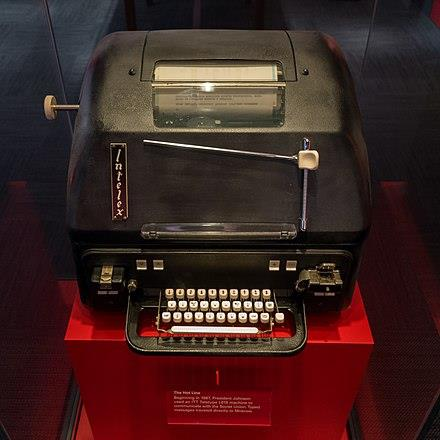
\includegraphics[width=0.85\textwidth]{../../images/python/page_024_img_01.jpeg}

% deskripsi: gambar native xref 117
\noindent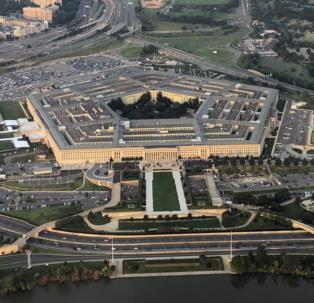
\includegraphics[width=0.85\textwidth]{../../images/python/page_024_img_02.jpeg}

% deskripsi: gambar native xref 118
\noindent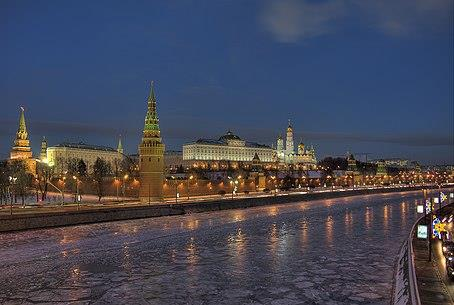
\includegraphics[width=0.85\textwidth]{../../images/python/page_024_img_03.jpeg}

\end{document}
